% ═══════════════════════════════════════════════════════════════
% ANSWER KEY: Horizontal Projectile Motion (Physics Grade 10E)
% E-Course Advanced Level (★★★)
% ═══════════════════════════════════════════════════════════════

\documentclass[10pt, a4paper]{article}

% ═══════════════════════════════════════════════════════════════
% PACKAGES
% ═══════════════════════════════════════════════════════════════

\usepackage[utf8]{inputenc}
\usepackage[T1]{fontenc}
\usepackage[english]{babel}
\usepackage{helvet}
\renewcommand{\familydefault}{\sfdefault}

\usepackage[margin=1.5cm, top=1.8cm, bottom=1.5cm]{geometry}
\usepackage{enumitem}
\usepackage{tabularx}
\usepackage{booktabs}
\usepackage{array}
\usepackage{multicol}
\usepackage{amsmath}
\usepackage{amssymb}

\usepackage{xcolor}
\usepackage{tcolorbox}
\usepackage{fancyhdr}
\usepackage{lastpage}
\usepackage{tikz}

% Compact lists
\setlist{nosep, leftmargin=1.5em}

% ═══════════════════════════════════════════════════════════════
% COLORS
% ═══════════════════════════════════════════════════════════════

\definecolor{physik}{HTML}{2c5aa0}
\definecolor{grau}{HTML}{888888}
\definecolor{hellgrau}{HTML}{f0f0f0}
\definecolor{success}{HTML}{2a7a4b}
\definecolor{warning}{HTML}{b35c00}
\definecolor{loesung}{HTML}{c62828}

\newcommand{\fachfarbe}{physik}

% ═══════════════════════════════════════════════════════════════
% VARIABLES
% ═══════════════════════════════════════════════════════════════

\newcommand{\thema}{Horizontal Projectile Motion}
\newcommand{\fach}{Physics}
\newcommand{\klasse}{Grade 10E}
\newcommand{\stunde}{Kinematics}

% ═══════════════════════════════════════════════════════════════
% HEADER AND FOOTER
% ═══════════════════════════════════════════════════════════════

\pagestyle{fancy}
\fancyhf{}
\renewcommand{\headrulewidth}{0.4pt}
\renewcommand{\footrulewidth}{0pt}

\lhead{\small\fach{} \klasse{} -- \thema{} \textcolor{loesung}{\textbf{(ANSWER KEY)}}}
\rhead{\small}

\cfoot{\small\thepage/\pageref{LastPage}}

% ═══════════════════════════════════════════════════════════════
% COMMANDS
% ═══════════════════════════════════════════════════════════════

% Solution (red)
\newcommand{\lsg}[1]{\textcolor{loesung}{\textbf{#1}}}

% Physics highlight
\newcommand{\ph}[1]{\textcolor{\fachfarbe}{\textbf{#1}}}

% Difficulty stars
\newcommand{\stmark}{$\star$}

% Key concept box
\newtcolorbox{merksatz}[1][]{
    colback=hellgrau,
    colframe=\fachfarbe,
    boxrule=0.8pt,
    arc=0pt,
    left=6pt, right=6pt, top=6pt, bottom=6pt,
    fonttitle=\bfseries\small,
    title=#1
}

% Formula box
\newtcolorbox{formelbox}{
    colback=white,
    colframe=\fachfarbe,
    boxrule=1.5pt,
    arc=0pt,
    left=8pt, right=8pt, top=8pt, bottom=8pt
}

% Note box
\newtcolorbox{hinweisbox}{
    colback=white,
    colframe=warning,
    boxrule=1pt,
    arc=0pt,
    left=6pt, right=6pt, top=6pt, bottom=6pt
}

% Section title
\newcommand{\abschnitt}[1]{%
    \vspace{8pt}
    \noindent\textbf{\textcolor{\fachfarbe}{#1}}
    \vspace{4pt}
}

% Points marker
\newcommand{\punkte}[1]{\hfill\small\textcolor{grau}{/#1 pts}}

% ═══════════════════════════════════════════════════════════════
% DOCUMENT
% ═══════════════════════════════════════════════════════════════

\begin{document}

% ═══════════════════════════════════════════════════════════════
% TITLE
% ═══════════════════════════════════════════════════════════════

\begin{center}
{\large\bfseries Worksheet: \thema{} -- \textcolor{loesung}{ANSWER KEY}}\\[2pt]
{\small\textcolor{grau}{Solutions in red}}
\end{center}

\vspace{-2pt}
\hrule
\vspace{8pt}

% ═══════════════════════════════════════════════════════════════
% TWO-COLUMN LAYOUT
% ═══════════════════════════════════════════════════════════════

\begin{multicols}{2}
\small

% ─────────────────────────────────────────────────────────────
% BOX 1: Key Insight
% ─────────────────────────────────────────────────────────────

\abschnitt{Box 1: The Principle of Superposition}

\begin{merksatz}[Key Concept]
In horizontal projectile motion, two \ph{independent} motions are superimposed:

\vspace{6pt}
\begin{tabular}{ll}
\textbf{Horizontal:} & \lsg{uniform} motion \\[4pt]
\textbf{Vertical:} & \lsg{free fall} \\
\end{tabular}

\vspace{8pt}
The horizontal velocity does \textbf{not} affect the

\lsg{fall time}.

\vspace{6pt}
Therefore, a falling ball and a thrown ball,

starting simultaneously, land \lsg{at the same time}.
\end{merksatz}

\vspace{4pt}

% ─────────────────────────────────────────────────────────────
% DIAGRAM
% ─────────────────────────────────────────────────────────────

\abschnitt{Diagram: Trajectory with Velocities}

\begin{center}
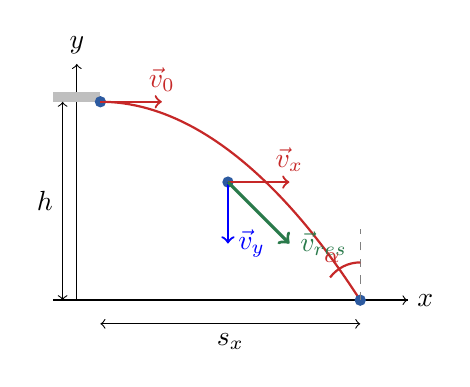
\begin{tikzpicture}[scale=0.6]
    % Coordinate system
    \draw[->] (0,0) -- (7,0) node[right] {$x$};
    \draw[->] (0,0) -- (0,5) node[above] {$y$};

    % Ground
    \draw[thick] (-0.5,0) -- (7,0);

    % Platform
    \fill[gray!50] (-0.5,4.2) rectangle (0.5,4.4);

    % Height h
    \draw[<->] (-0.3,0) -- (-0.3,4.2) node[midway, left] {$h$};

    % Parabola (red for solution)
    \draw[thick, loesung] (0.5,4.2) parabola (6,0);

    % Ball start
    \fill[physik] (0.5,4.2) circle (0.12);

    % Ball middle
    \fill[physik] (3.2,2.5) circle (0.12);

    % Ball end
    \fill[physik] (6,0) circle (0.12);

    % Range
    \draw[<->] (0.5,-0.5) -- (6,-0.5) node[midway, below] {$s_x$};

    % v0 arrow (start)
    \draw[->, thick, loesung] (0.5,4.2) -- (1.8,4.2) node[above] {$\vec{v}_0$};

    % v_x arrow (middle) - horizontal
    \draw[->, thick, loesung] (3.2,2.5) -- (4.5,2.5) node[above] {$\vec{v}_x$};

    % v_y arrow (middle) - vertical downward
    \draw[->, thick, blue] (3.2,2.5) -- (3.2,1.2) node[right] {$\vec{v}_y$};

    % v_res arrow (middle) - diagonal
    \draw[->, very thick, success] (3.2,2.5) -- (4.5,1.2) node[right] {$\vec{v}_{res}$};

    % Impact angle at end
    \draw[dashed, gray] (6,0) -- (6,1.5);
    \draw[thick, loesung] (6,0.8) arc (90:143:0.8);
    \node at (5.4,0.9) {\footnotesize\lsg{$\alpha$}};
\end{tikzpicture}
\end{center}

% ─────────────────────────────────────────────────────────────
% BOX 2: Basic Formulas
% ─────────────────────────────────────────────────────────────

\abschnitt{Box 2: Basic Formulas}

\begin{formelbox}
\textbf{Step 1: Time of Flight}
\vspace{2pt}

\begin{equation*}
t = \sqrt{\frac{2h}{g}}
\end{equation*}

\vspace{2pt}
\footnotesize
$t$ = time [s] \quad $h$ = height [m] \quad $g \approx 10\,\text{m/s}^2$
\end{formelbox}

\vspace{4pt}

\begin{formelbox}
\textbf{Step 2: Horizontal Range}
\vspace{2pt}

\begin{equation*}
s_x = v_0 \cdot t
\end{equation*}

\vspace{2pt}
\footnotesize
$s_x$ = range [m] \quad $v_0$ = initial velocity [m/s]
\end{formelbox}

\vspace{4pt}

% ─────────────────────────────────────────────────────────────
% BOX 3: Advanced Formulas
% ─────────────────────────────────────────────────────────────

\abschnitt{Box 3: Advanced Formulas (E-Course)}

\begin{formelbox}
\textbf{Vertical Velocity at Impact}
\vspace{2pt}

\begin{equation*}
v_y = g \cdot t
\end{equation*}

\vspace{2pt}
\footnotesize
$v_y$ = vertical velocity at impact [m/s]
\end{formelbox}

\vspace{4pt}

\begin{formelbox}
\textbf{Resultant Velocity}
\vspace{2pt}

\begin{equation*}
v_{res} = \sqrt{v_x^2 + v_y^2}
\end{equation*}

\vspace{2pt}
\footnotesize
$v_{res}$ = impact velocity [m/s] \quad (Pythagorean theorem!)
\end{formelbox}

\vspace{4pt}

\begin{formelbox}
\textbf{Impact Angle}
\vspace{2pt}

\begin{equation*}
\tan(\alpha) = \frac{v_y}{v_x} \quad \Rightarrow \quad \alpha = \arctan\left(\frac{v_y}{v_x}\right)
\end{equation*}

\vspace{2pt}
\footnotesize
$\alpha$ = angle to horizontal at impact
\end{formelbox}

\vspace{4pt}

\begin{hinweisbox}
\footnotesize
\textbf{Note:} We calculate with $g \approx 10\,\text{m/s}^2$ for simple numbers.\\
The exact value is $g = 9.81\,\text{m/s}^2$.
\end{hinweisbox}

% ─────────────────────────────────────────────────────────────
% Column break
% ─────────────────────────────────────────────────────────────

\columnbreak

% ─────────────────────────────────────────────────────────────
% TABLE
% ─────────────────────────────────────────────────────────────

\abschnitt{Table: Typical Fall Times}

\begin{center}
\begin{tabular}{|c|c|}
\hline
\textbf{Height $h$} & \textbf{Fall time $t$} \\
\hline
5 m & 1 s \\
\hline
20 m & 2 s \\
\hline
45 m & 3 s \\
\hline
80 m & 4 s \\
\hline
\end{tabular}
\end{center}

\vspace{2pt}

% ─────────────────────────────────────────────────────────────
% PROBLEM 1 WITH SOLUTION
% ─────────────────────────────────────────────────────────────

\abschnitt{Problem 1: Basic (\stmark\stmark)}\punkte{4}

A ball is thrown horizontally from $h = 20\,\text{m}$ with $v_0 = 15\,\text{m/s}$.

\textbf{a)} Calculate the time of flight.

\textcolor{loesung}{$t = \sqrt{\dfrac{2h}{g}} = \sqrt{\dfrac{2 \cdot 20\,\text{m}}{10\,\text{m/s}^2}} = \sqrt{4\,\text{s}^2}$ \quad $\boxed{t = 2\,\text{s}}$}

\vspace{4pt}

\textbf{b)} Calculate the horizontal range.

\textcolor{loesung}{$s_x = v_0 \cdot t = 15\,\text{m/s} \cdot 2\,\text{s}$ \quad $\boxed{s_x = 30\,\text{m}}$}

\vspace{4pt}

% ─────────────────────────────────────────────────────────────
% PROBLEM 2 WITH SOLUTION
% ─────────────────────────────────────────────────────────────

\abschnitt{Problem 2: Application (\stmark\stmark)}\punkte{5}

An airplane flies at $h = 45\,\text{m}$ with $v_0 = 20\,\text{m/s}$. It drops a supply package.

\textbf{a)} How long is the package in the air?

\textcolor{loesung}{$t = \sqrt{\dfrac{2 \cdot 45\,\text{m}}{10\,\text{m/s}^2}} = \sqrt{9\,\text{s}^2}$ \quad $\boxed{t = 3\,\text{s}}$}

\vspace{4pt}

\textbf{b)} How far before the target must it be released?

\textcolor{loesung}{$s_x = 20\,\text{m/s} \cdot 3\,\text{s}$ \quad $\boxed{s_x = 60\,\text{m}}$}

\vspace{4pt}

% ─────────────────────────────────────────────────────────────
% PROBLEM 3 WITH SOLUTION
% ─────────────────────────────────────────────────────────────

\abschnitt{Problem 3: Advanced (\stmark\stmark\stmark)}\punkte{8}

A cliff diver jumps from $h = 80\,\text{m}$ with $v_0 = 30\,\text{m/s}$.

\textbf{a)} Calculate the time of flight $t$.

\textcolor{loesung}{$t = \sqrt{\dfrac{2 \cdot 80}{10}}\,\text{s} = \sqrt{16}\,\text{s} = \boxed{4\,\text{s}}$}

\vspace{2pt}

\textbf{b)} Calculate the horizontal range $s_x$.

\textcolor{loesung}{$s_x = 30\,\text{m/s} \cdot 4\,\text{s} = \boxed{120\,\text{m}}$}

\vspace{2pt}

\textbf{c)} Calculate the vertical velocity $v_y$ at impact.

\textcolor{loesung}{$v_y = g \cdot t = 10\,\text{m/s}^2 \cdot 4\,\text{s} = \boxed{40\,\text{m/s}}$}

\vspace{2pt}

\textbf{d)} Calculate the impact velocity $v_{res}$.

\textcolor{loesung}{$v_{res} = \sqrt{v_x^2 + v_y^2} = \sqrt{30^2 + 40^2}\,\text{m/s} = \sqrt{2500}\,\text{m/s}$ \quad $\boxed{v_{res} = 50\,\text{m/s}}$ (3-4-5 triangle!)}

\vspace{4pt}

% ─────────────────────────────────────────────────────────────
% PROBLEM 4 WITH SOLUTION
% ─────────────────────────────────────────────────────────────

\abschnitt{Problem 4: Transfer (\stmark\stmark\stmark)}\punkte{6}

A stuntman jumps from a rooftop and lands $s_x = 90\,\text{m}$ away with $v_{res} = 50\,\text{m/s}$.

\textbf{a)} Calculate $v_0$ if $v_y = 40\,\text{m/s}$.

\textcolor{loesung}{Pythagorean theorem reversed: $v_{res}^2 = v_0^2 + v_y^2$ $\Rightarrow$ $v_0 = \sqrt{v_{res}^2 - v_y^2} = \sqrt{50^2 - 40^2}\,\text{m/s} = \sqrt{900}\,\text{m/s}$ \quad $\boxed{v_0 = 30\,\text{m/s}}$}

\vspace{2pt}

\textbf{b)} Calculate the time of flight $t$.

\textcolor{loesung}{Rearranging: $s_x = v_0 \cdot t \Rightarrow t = \dfrac{s_x}{v_0}$ \quad $t = \dfrac{90\,\text{m}}{30\,\text{m/s}} = \boxed{3\,\text{s}}$}

\end{multicols}

% ═══════════════════════════════════════════════════════════════
% SELF-CHECK
% ═══════════════════════════════════════════════════════════════

\vspace{4pt}
\hrule
\vspace{6pt}

\small
\textbf{Self-Check -- I can...}

\begin{tabular}{|p{6cm}|c|c||p{6cm}|c|c|}
\hline
\textbf{Competency} & \textbf{Yes} & \textbf{No} & \textbf{Competency} & \textbf{Yes} & \textbf{No} \\
\hline
...explain why both balls land simultaneously. & \lsg{$\boxtimes$} & $\square$ &
...calculate the impact velocity $v_{res}$. & \lsg{$\boxtimes$} & $\square$ \\
\hline
...calculate the fall time from height. & \lsg{$\boxtimes$} & $\square$ &
...calculate the impact angle $\alpha$. & \lsg{$\boxtimes$} & $\square$ \\
\hline
...calculate the horizontal range. & \lsg{$\boxtimes$} & $\square$ &
...analyze real-world applications. & \lsg{$\boxtimes$} & $\square$ \\
\hline
\end{tabular}

% ═══════════════════════════════════════════════════════════════
% POINTS OVERVIEW
% ═══════════════════════════════════════════════════════════════

\vfill
\hrule
\vspace{4pt}
\small
\begin{tabular}{llllll}
\textbf{Problem 1:} & \lsg{4} / 4 pts &
\textbf{Problem 2:} & \lsg{5} / 5 pts &
\textbf{Problem 3:} & \lsg{8} / 8 pts \\[4pt]
\textbf{Problem 4:} & \lsg{6} / 6 pts &
\textbf{Total:} & \lsg{23} / 23 pts &
\textbf{Grade:} & \lsg{15 pts / A}
\end{tabular}

\end{document}
